\beginsong{Drei glänzende Kugeln}[
    wuw={Franz Joseph Degenhardt},
    jahr={1963}, 
    bo={126}, 
    pfii={34}, 
    pfiii={15}, 
    kssiv={14}, 
    siru={74}, 
    tonspur={258}, 
    index={Es liegen drei glänzende Kugeln},
]

\beginverse
\endverse
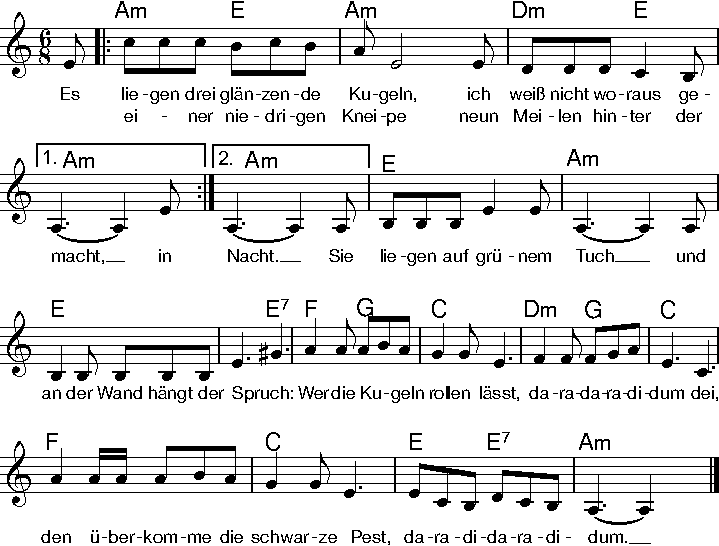
\includegraphics[draft=false, width=1\textwidth]{Noten/Lied038.pdf}	

\beginverse
Der \[Am]Wirt, der \[E]hat nur ein \[Am]Auge und \[Dm]das trägt er \[E]hinter dem \[Am]Ohr.
Aus seinem ge\[E]spaltenen \[Am]Kopfe ragt \[Dm]eine An\[E]tenne her\[Am]vor.
Er \[E]trinkt aus einer \[Am]Seele und \[E]ruft aus roter Keh\[E7]le:
\endverse

\beginchorus
\[F]Wer die Kugeln \[C]rollen lässt, \[Dm]daradaradi\[C]dum dei,
\[F]den überkomme die \[C]schwarze Pest, \[E]dara\[E7]daradi\[Am]dum.
\endchorus

\beginverse
Die ^einen ^sagen, die ^Kugeln sind die ^Sonne, die ^Erde, der ^Mond.
Die anderen ^glauben, sie ^seien das ^Feuer, die ^Angst und der ^Tod.
Und ^wenn sie beisammen ^sind, dann ^summen sie in den ^Wind:
\endverse

\beginchorus
\[F]Wer die Kugeln \[C]rollen lässt, \[Dm]daradaradi\[C]dum dei,
\[F]den überkomme die \[C]schwarze Pest, \[E]dara\[E7]daradi\[Am]dum.
\endchorus

\beginverse
Und ^dann kam ^einer ge^ritten, es ^war in dem ^Jahr vor der ^Zeit,
auf einer ^gesattelten ^Wolke von ^hinter der ^Ewig^keit.
Er ^nahm von der Wand einen ^Queue, der ^Wirt rief krächzend: ''He, ^he!''
\endverse

\printchorus

\beginverse
Doch ^jener, der ^lachte zwei ^Donner und ^wachste den ^knöchernen ^Stab,
visierte und ^stieß, und die ^Kugeln prallten ^aneinander, der ^Wirt grub sein ^Grab.
^Fäulnis flatterte ^auf, so ^nahm alles seinen ^Lauf.
\endverse

\printchorus

\endsong

\beginscripture{}
Das Lied, eines der frühesten Degenhardts, erschien erstmals auf seiner Platte "Zwischen Null Uhr Null und Mitternacht" (1963). Ein Interpretationsansatz geht davon aus, dass in dem Lied das Forschen mit Atomenergie kritisiert wird. So könnten die Kugeln für die Atome stehen, die vom Menschen nicht angestoßen werden sollen, und der verunstaltete Wirt für die möglichen gesundheitlichen Folgen des Experimentierens mit Atomenergie.
\endscripture
